\chapter{Análisis de resultados}

A lo largo de este capítulo se mostrarán los resultados obtenidos del experimento planteado tal y como se ha diseñado en el apartado anterior. Se construirán en primer lugar las tablas que recojan los valores obtenidos por cada algoritmo en cada una de las distintas situaciones planteadas, y a continuación, con ayuda de gráficas, se visualizarán de forma más clara estos valores, para así poder sacar conclusiones más fácilmente.

En primer lugar se muestran las tablas con los resultados de los grupos de colegas y aleatorios respectivamente. Se muestran los datos obtenidos con la métrica \textbf{NDCG}, situándose en un rango [0,1]. Se disponen los resultados para cada algoritmo y estrategia de combinación, donde \textit{AVG} representa la estrategia de la media, \textit{MIN} la del mínimo, \textit{MAX} la del máximo y \textit{MAJ} la de la mayoría.

Se separará la tabla en tres apartados: en primer lugar aparecerá el algoritmo \textit{baseline}, como modelo base con el que comparar en primera instancia; en segundo lugar aparecerá el algoritmo POGRS del estado del arte, como modelo actual a batir; y por último, se mostrarán las 4 propuestas del estudio para que se puedan comparar directamente entre ellas, pero también con los resultados obtenidos por los algoritmos de referencia anteriormente mencionados.

En la tabla \ref{t:resultados-colegas} se muestran los resultados de los grupos de colegas, mientras que en la tabla \ref{t:resultados-aleatorios} se muestran los de los grupos aleatorios.

\begin{table}[H]
	\centering
	\begin{tabular}{ccccc}
		\toprule
		{} & \textbf{AVG} & \textbf{MIN} & \textbf{MAX} & \textbf{MAJ} \\
		\midrule
		\textbf{Baseline} & 8.3419e-01 & 8.2756e-01 & 8.4632e-01 & 8.2171e-01 \\
		\midrule
		\textbf{POGRS} & \textbf{8.4692e-01} & \textbf{8.6989e-01} & \textbf{8.5375e-01} & \textbf{8.5069e-01} \\
		\midrule
		\textbf{Empatía} & 8.3920e-01 & 8.2197e-01 & 8.3857e-01 & 8.2872e-01 \\
		\textbf{Cinéfilo} & 8.4016e-01 & 8.3195e-01 & 8.4802e-01 & 8.2597e-01 \\
		\textbf{Optimista} & 8.4296e-01 & 8.2019e-01 & 8.3477e-01 & 8.1591e-01 \\
		\textbf{Similitud} & 8.4264e-01 & 8.4975e-01 & 8.4690e-01 & 8.3506e-01 \\
		\bottomrule
	\end{tabular}
	\caption{Resultados obtenidos utilizando grupos de colegas.}
	\label{t:resultados-colegas}
\end{table}

\begin{table}[H]
	\centering
	\begin{tabular}{ccccc}
		\toprule
		{} & \textbf{AVG} & \textbf{MIN} & \textbf{MAX} & \textbf{MAJ} \\
		\midrule
		\textbf{Baseline} & 8.51552e-01 & 8.60739e-01 & 8.61638e-01 & 8.73572e-01 \\
		\midrule
		\textbf{POGRS} & \textbf{8.72791e-01} & \textbf{9.13770e-01} & \textbf{8.97229e-01} & \textbf{8.82410e-01} \\
		\midrule
		\textbf{Empatía} & 8.50348e-01 & 8.58027e-01 & 8.59491e-01 & 8.58129e-01 \\
		\textbf{Cinéfilo} & 8.54243e-01 & 8.67626e-01 & 8.63351e-01 & 8.60463e-01 \\
		\textbf{Optimista} & 8.56988e-01 & 8.64129e-01 & 8.64698e-01 & 8.54955e-01 \\
		\textbf{Similitud} & 8.66558e-01 & 8.93580e-01 & 8.78917e-01 & 8.73205e-01 \\
		\bottomrule
	\end{tabular}
	\caption{Resultados obtenidos utilizando grupos aleatorios.}
	\label{t:resultados-aleatorios}
\end{table}

Una vez expuestos los resultados del experimento, se complementan con dos gráficas que permiten visualizar de manera más clara la diferencia en términos de eficacia de cada uno de los métodos para cada estrategia de combinación.

En la figura \ref{grafica-colegas} se puede visualizar el rendimiento de los algoritmos para los grupos de colegas, y en la figura \ref{grafica-aleatorios} para los grupos aleatorios.

\begin{figure}[H]
	\centering
	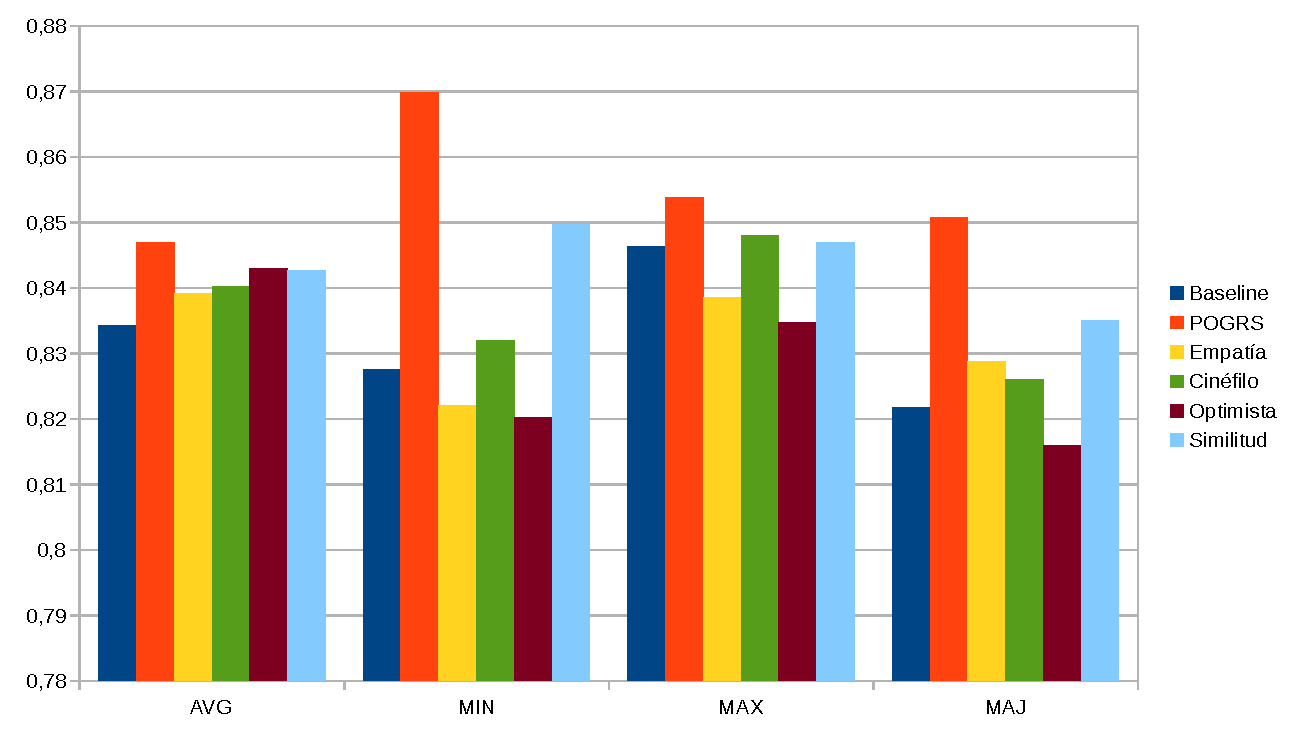
\includegraphics[scale=0.6]{imagenes/grafica-colegas.pdf}
	\caption{Histograma agrupado por estrategia de combinación para grupos de colegas.}
	\label{grafica-colegas}
\end{figure}

\begin{figure}[H]
	\centering
	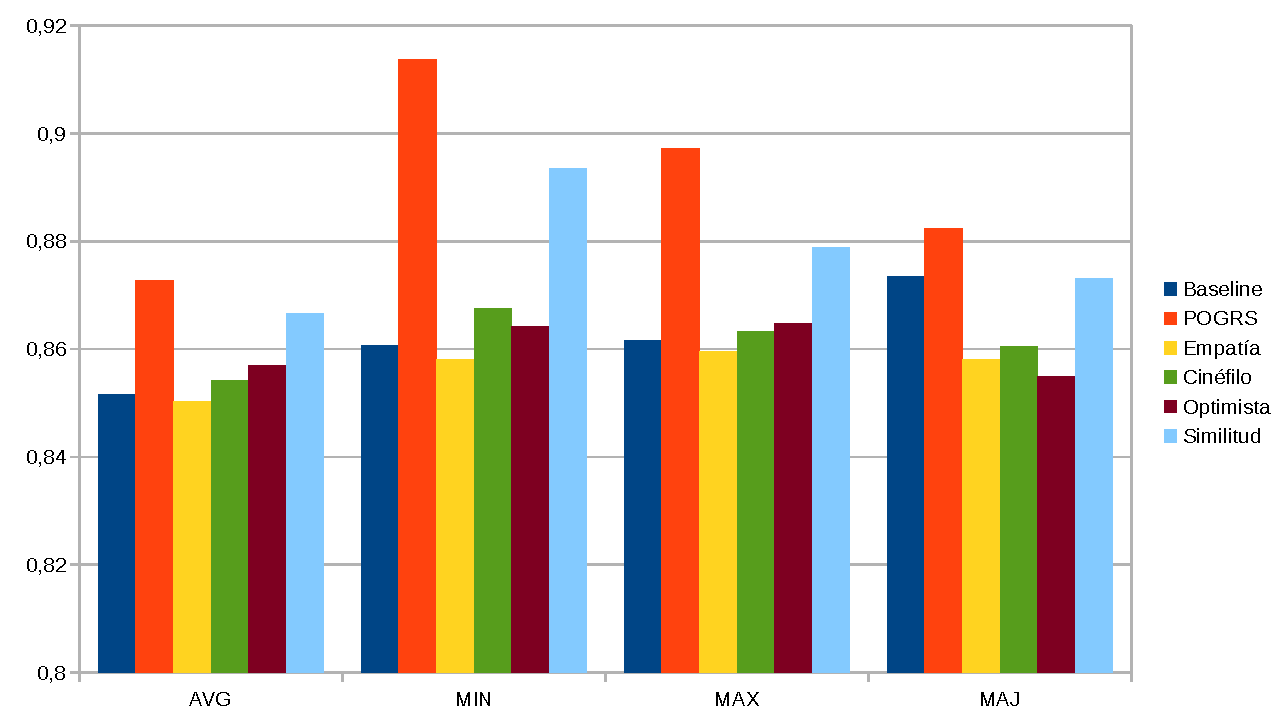
\includegraphics[scale=0.6]{imagenes/grafica-aleatorios.pdf}
	\caption{Histograma agrupado por estrategia de combinación para grupos aleatorios.}
	\label{grafica-aleatorios}
\end{figure}

A continuación se procede a realizar el análisis sobre los resultados recopilados, considerando tanto las tablas como las gráficas para poder realizar conjeturas y extraer conclusiones de los mismos.

Partiendo de una comparación directa entre las 4 nuevas propuestas planteadas en este estudio, destaca de forma general el rendimiento de una de ella por encima del resto: se trata del método \textbf{de mayor similitud}. Por supuesto que mirando las gráficas se puede percibir que no en todos los casos particulares resulta ser el mejor, pero sí que lo es en la mayoría (además mediante diferencias considerablamente amplias), y en los que no lo logra se encuentra muy cerca.

En cuanto al resto de las propuestas planteadas, no existe una diferencia significativa entre ellas, dándose casos donde resulta ser mejor la propuesta de empatía (en la combinación MAJ para grupos de colegas), otros en los que lo es mejor la propuesta del más cinéfilo, y con bastante diferencia (combinaciones MIN y MAX para grupos de colegas), y por último otros en los que la mejor de las tres resulta ser la propuesta del más optimista (la combinación MAX para grupos aleatorios y la AVG para ambos tipos de grupos).

Para visualizar mejor estas clasificaciones se puede hacer una tabla con el ranking que obtiene cada método para cada una de las estrategias de combinación. Además, se adjunta una columna adicional que recoja el valor medio de su posición en cada estrategia para finalmente obtener una valoración general de dicho algoritmo.

\begin{table}[H]
	\centering
	\begin{tabular}{ccccc|c}
		\toprule
		{} & \textbf{AVG} & \textbf{MIN} & \textbf{MAX} & \textbf{MAJ} & \textbf{Pos. Media} \\
		\midrule
		\textbf{Baseline} & 6 & 4 & 4 & 5 & 4.75 \\
		\midrule
		\textbf{POGRS} & \textbf{1} & \textbf{1} & \textbf{1} & \textbf{1} & \textbf{1} \\
		\midrule
		\textbf{Empatía} & 5 & 5 & 5 & 3 & 4.5 \\
		\textbf{Cinéfilo} & 4 & 3 & 2 & 4 & 3.25 \\
		\textbf{Optimista} & 2 & 6 & 6 & 6 & 5 \\
		\textbf{Similitud} & 3 & 2 & 3 & 2 & 2.5 \\
		\bottomrule
	\end{tabular}
	\caption{Posición obtenida por los métodos utilizando grupos de colegas.}
	\label{t:posicion-colegas}
\end{table}

\begin{table}[H]
	\centering
		\begin{tabular}{ccccc|c}
			\toprule
			{} & \textbf{AVG} & \textbf{MIN} & \textbf{MAX} & \textbf{MAJ} & \textbf{Pos. Media} \\
			\midrule
			\textbf{Baseline} & 5 & 5 & 5 & 2 & 4.25 \\
			\midrule
			\textbf{POGRS} & \textbf{1} & \textbf{1} & \textbf{1} & \textbf{1} & \textbf{1} \\
			\midrule
			\textbf{Empatía} & 6 & 6 & 6 & 5 & 5.75 \\
			\textbf{Cinéfilo} & 4 & 3 & 4 & 4 & 3.75 \\
			\textbf{Optimista} & 3 & 4 & 3 & 6 & 4 \\
			\textbf{Similitud} & 2 & 2 & 2 & 3 & 2.25 \\
			\bottomrule
	\end{tabular}
	\caption{Posición obtenida por los métodos utilizando grupos aleatorios.}
	\label{t:posicion-aleatorios}
\end{table}

En la tabla del ranking destaca primeramente que el POGRS es con diferencia el mejor método de los que se han evaluado en el estudio. Si se comparan las dos tablas (colegas y aleatorios) se observa que además el algoritmo de similitud es siempre el segundo mejor algoritmo, quedando representada de forma numérica la hipótesis que se planteó observando la gráfica, y por tanto es la mejor de las nuevas propuestas planteadas para este trabajo. Estos dos datos ya se habían intuido previamente con sólo mirar a la gráfica, pero con la nueva tabla se puede debatir con más información la eficacia del resto de métodos entre sí.

La técnica del más cinéfilo se sitúa por encima de las dos propuestas restantes en el ranking general, tanto para los grupos de colegas como para los aleatorios, ocupando la tercera posición del ranking por detrás del POGRS y del algoritmo de mayor similitud. Gracias a esto se puede confirmar que es el segundo mejor de los métodos ideados e implementados para este estudio. Referente a los otros dos, el método de empatía y el del más optimista, existe un poco más de debate.

Para empezar, conviene realizar una comparativa con el algoritmo \textit{baseline}. Este algoritmo por lo general es simple y no ofrece resultados muy óptimos, y como se puede comprobar tanto el POGRS como el de mayor similitud le superan de forma habitual (excepto en el caso de combinación MAJ para grupos aleatorios, en el que el \textit{baseline} se comporta inusualmente bien). Sin embargo, no queda igual de clara la comparativa con los otros dos métodos propuestos. Se comporta a menudo de manera inconsistente, variando entre puntuaciones altas situándose de las primeras posiciones a ocupar la última o penúltima en otros cuantos casos. Esto provoca que su posición media a raíz de los resultados obtenidos esté rondando el 4, con 4.75 sobre 6 para los grupos de colegas y 4.25 sobre 6 para grupos aleatorios. A continuación se realizará su comparativa con las dos nuevas propuestas restantes para ambos tipos de grupos.

En el caso de los grupos aleatorios, el método de empatía obtiene resultados particularmente malos, quedando en último lugar en 3 de las 4 estrategias de combinación y obteniendo casi un 6 sobre 6 en el ranking de posición media. Este ranking sin embargo mejora para los grupos de colegas, donde el método de empatía sube hasta un 4.5 sobre 6, colocándose por delante de los métodos \textit{baseline} y del más optimista.

En cuanto al método del más optimista, sigue un patrón un poco contrario al de empatía; en este caso, para los grupos de colegas ocupa la peor posición en 3 de las 4 estrategias de combinación, pero sin embargo resulta la segunda mejor propuesta en la combinación AVG. Al final, su posición media para este tipo de grupos es de 5 sobre 6, quedando relegada a la peor propuesta en esta configuración del experimento. Para grupos aleatorios, sin embargo, su eficacia es más difícil de seguir puesto que en algunos casos ocupa la peor posición y en otras por el contrario se sitúa por encima de la media, quedando en un 4 sobre 6 como posición media.

En comparación con el algoritmo \textit{baseline}, el método de empatía resulta ser peor con bastante diferencia para los casos de grupos aleatorios, y solamente se comporta ligeramente mejor para grupos de colegas. Estos resultados dan a entender que este método sale bastante perjudicado del estudio, ya que es incapaz de competir ni siquiera con el algoritmo más básico de los propuestos. En cuanto al método del más optimista, es ligeramente superior al \textit{baseline} para grupos aleatorios pero también ligeramente inferior para grupos de colegas, quedando igualmente en una posición un poco comprometida. Analizando sus resultados y basándose en los rankings generados a partir de las tablas, se puede afirmar que tiene un comportamiento en general bastante similar a este algoritmo en cuanto a los términos del experimento se refiere.